\documentclass{amsart}

\usepackage[brazilian]{babel}
\usepackage[utf8]{inputenc}
\usepackage{graphicx}
\usepackage{mathtools}
\usepackage{amsthm}
\usepackage{thmtools,thm-restate}
\usepackage{amsfonts}
\usepackage{hyperref}
\usepackage[singlelinecheck=false]{caption}
\usepackage[backend=biber,url=true,doi=true,eprint=false,style=alphabetic]{biblatex}
\usepackage{enumitem}
\usepackage[justification=centering]{caption}
\usepackage{indentfirst}
\usepackage{algorithm}
\usepackage{algpseudocode}
\usepackage{listings}

\addbibresource{references.bib}

\makeatletter
\def\subsection{\@startsection{subsection}{3}%
  \z@{.5\linespacing\@plus.7\linespacing}{.1\linespacing}%
  {\normalfont\itshape}}
\makeatother

\DeclareMathOperator*{\argmin}{arg\,min}
\DeclareMathOperator*{\argmax}{arg\,max}

\newcommand\defeq{\mathrel{\overset{\makebox[0pt]{\mbox{\normalfont\tiny\sffamily def}}}{=}}}

\floatname{algorithm}{Algoritmo}
\algrenewcommand\algorithmicrequire{\textbf{Input}}
\algrenewcommand\algorithmicensure{\textbf{Output}}
\algtext*{EndIf}
\algtext*{EndFunction}
\algtext*{EndWhile}

\captionsetup[table]{labelsep=space}

\theoremstyle{plain}

\newcounter{dummy-def}\numberwithin{dummy-def}{section}
\newtheorem{definition}[dummy-def]{Definição}
\newcounter{dummy-thm}\numberwithin{dummy-thm}{section}
\newtheorem{theorem}[dummy-thm]{Teorema}
\newcounter{dummy-prop}\numberwithin{dummy-prop}{section}
\newtheorem{proposition}[dummy-prop]{Proposição}
\newcounter{dummy-ex}\numberwithin{dummy-ex}{section}
\newtheorem{exercise}[dummy-ex]{Exercício}
\newcounter{dummy-eg}\numberwithin{dummy-eg}{section}
\newtheorem{example}[dummy-eg]{Exemplo}

\numberwithin{equation}{section}

\newcommand{\set}[1]{\mathbf{#1}}
\newcommand{\pr}{\mathbb{P}}
\renewcommand{\implies}{\Rightarrow}

\newcommand{\bigo}{\mathcal{O}}

\setlength{\parskip}{1em}

\lstset{frameround=fttt,
  language=[5.3]Lua,
	numbers=left,
	breaklines=true,
	keywordstyle=\bfseries,
	basicstyle=\ttfamily,
}

\newcommand{\code}[1]{\lstinline[mathescape=true]{#1}}
\newcommand{\mcode}[1]{\lstinline[mathescape]!#1!}


\title{%
  \noindent\rule{10cm}{0.8pt}\\
  Prova 2\\[1ex]
  \scriptsize\mdseries
  MAC0438 - Programação Concorrente\\
  Instituto de Matemática e Estatística - USP\\%
  \tiny~\\
  $1^\text{o}$ Semestre de 2016 - Prof. Marcel P. Jackowski\\%
  \noindent\rule{10cm}{0.8pt}
}
\xdef\shorttitle{P2 MAC0438 - Renato Geh}
%\title[]{Estudo sobre Sum-Product Networks e Aprendizagem Profunda}
\author[]{Renato Lui Geh\\NUSP\@: 8536030}

\begin{document}

\maketitle

\section*{Questão 1}

A Figura~\ref{ex1-fig} ilustra as dependências $D=\{P_1\to P_2, P_1\to P_3, P_2\to P_4, P_3\to
P_5, P_4\to P_5\}$. Uma aresta direcionada indica uma dependência em $D$. Uma aresta
não-direcionada indica a necessidade de um semáforo $S_i$. A altura de um nó indica se precisamos
terminar algum processo antes. A altura do nó raíz $P_1$ é $h_1=0$, já que não temos nenhuma
dependência para $P_1$. Se um nó $i$ tem altura $h_i>0$, então precisamos completar todos os nós
que tenham altura menor que $h_i$. Por exemplo, para começarmos o processo $P_2$, precisamos
antes satisfazer a dependência $P_1$; para começarmos o processo $P_5$, precisamos completar os
nós $P_4$, $P_3$, $P_2$ e $P_1$ antes, já que estão em alturas menores que $P_5$.

\begin{figure}[h]
  \centering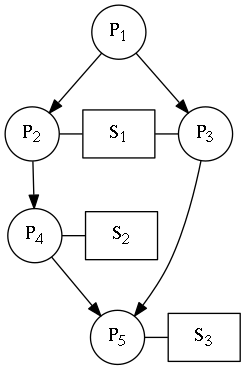
\includegraphics[scale=0.4]{graphs/ex1.png}
  \caption{}\label{ex1-fig}
\end{figure}

Portanto, sabemos do grafo quem devemos rodar antes de começarmos algum processo. O algoritmo
abaixo mostra o código de cada processo e a inicialização dos semáforos.

\begin{algorithm}
  \caption{}
  \begin{algorithmic}[1]
    \State~\texttt{sem} $S_1 \coloneqq 0$
    \State~\texttt{sem} $S_2 \coloneqq 0$
    \State~\texttt{sem} $S_3 \coloneqq -1$

    \Function{$P_1$:}{}
      \State~\texttt{código do processo 1}
      \State~$V(S_1)$
      \State~$V(S_1)$
    \EndFunction

    \Function{$P_2$:}{}
      \State~$P(S_1)$
      \State~\texttt{código do processo 2}
      \State~$P(S_2)$
    \EndFunction

    \Function{$P_3$:}{}
      \State~$P(S_1)$
      \State~\texttt{código do processo 3}
      \State~$P(S_3)$
    \EndFunction

    \Function{$P_4$:}{}
      \State~$P(S_2)$
      \State~\texttt{código do processo 4}
      \State~$P(S_3)$
    \EndFunction

    \Function{$P_5$:}{}
      \State~$P(S_3)$
      \State~$P(S_3)$
      \State~\texttt{código do processo 5}
    \EndFunction
  \end{algorithmic}
\end{algorithm}

\section*{Questão 2}

\begin{lstlisting}[mathescape=true]
  type s[1..M];  // Buffer
  int c = 0;
  sem write = 1;
  sem ready = 1;
  sem full = 0;

  produtor [i=1..N] { // Processos produtores
    P(write);
    P(ready);
    push(s[c]); // Deposita
    ++c;
    if (c == M) V(full);
    else V(ready);
    V(write);
  }

  consumidor { // Processo consumidor
    P(full);
    for (i $\gets$ 1..M)
      consume(S[i]); // Consome
    V(ready);
  }
\end{lstlisting}

\section*{Questão 3}

\begin{enumerate}[label=(\alph*)]
  \item Se por acesso exclusivo quer-se dizer que somente um processo poderá acessar a base de
    dados por vez, então não, o acesso não é exclusivo, já que os processos leitores podem ler a
    base de dados simultaneamente. No entanto, se considerarmos acesso exclusivo como a restrição
    de não haver leitura e escrita simultânea, então sim, há exclusão neste caso devido ao semáforo
    \code{escrita}. Como leitura simultânea não gera conflitos, não seria necessário
    sequencializar a leitura.
  \item \begin{itemize}
      \item \code{sem a = 1}\\
        Tem o propósito de controlar o acesso a variável global \code{nr}, que é modificada e lida
        em vários processos, e portanto requer exclusão mútua.
      \item \code{sem b = 1}\\
        Garante a exclusão mútua da variável \code{nw}. Análogo ao semáforo \code{a}.
      \item \code{sem c = 1}\\
        Semáforo que dá preferência a processos escritores (vide item c).
      \item \code{sem leitura = 1}\\
        Previne que processos leitores leiam a base de dados quando um processo escritos está
        modificando-a.
      \item \code{sem escrita = 1}\\
        Previne que processos escritores escrevam enquanto leitores lêem. Além disso, garante
        exclusão mútua entre múltiplos escritores.
      \item \code{int nr = 0}\\
        Contador de leitores ativos. Apenas o primeiro e último leitores travam e destravam os
        processos escritores.
      \item \code{int nw = 0}\\
        Análogo a \code{nr} para os escritores.
    \end{itemize}
  \item Esta solução dá preferência para os escritores devido ao semáforo \code{c}, já que este
    gasta o timeslice dos leitores com um semáforo para que os escritores possam ter mais tempo
    para escrita.
\end{enumerate}

\section*{Questão 4}

\begin{lstlisting}
  class semaphore {
    int i=0;
    cond c, k;

    void P() {
      wait(k);
      if (i == 0) wait(c);
      else ++i;
      signal(k);
    }

    void V() {
      wait(k);
      if (empty(c)) --i;
      else signal(c);
      signal(k);
    }
  }
\end{lstlisting}

%--------------------------------------------------------------------------------------------------

\newpage
\appendix

\newpage

\printbibliography[]

\end{document}
